\documentclass[doc,a4paper,12pt]{apa6}
\usepackage[a4paper]{geometry}
\usepackage[utf8]{inputenc}
\usepackage[T1]{fontenc}
\usepackage[ngerman]{babel}
\usepackage{amsmath}
\usepackage[doublespacing]{setspace}
\usepackage{paralist}
\usepackage{graphicx}
\usepackage{tabularx}
\usepackage{epstopdf}
\usepackage{wrapfig}
\usepackage{float}
\usepackage{csquotes}
\usepackage[hidelinks]{hyperref}
\usepackage{pdfpages}
\usepackage[backend=biber,style=apa]{biblatex}
\usepackage[titles]{tocloft}
\usepackage{subcaption}

\hypersetup{hidelinks}
\usepackage{letltxmacro}
\makeatletter
\AtBeginDocument{%
  \@ifdefinable{\myorg@nameref}{%
    \LetLtxMacro\myorg@nameref\nameref
    \DeclareRobustCommand*{\nameref}[1]{%
      \glqq{\myorg@nameref{#1}}\grqq%
    }%
  }%
}
\makeatother

\DeclareLanguageMapping{ngerman}{ngerman-apa}
\DefineBibliographyStrings{ngerman}{andothers={et\ al\adddot}}

\renewcommand{\arraystretch}{1.2}

\bibliography{references}
 
\title{Intrinsische Rauschunterdückung bei LCMV Beamformer und Minimum Norm Estimate bei Magnetenzephalographie}
\shorttitle{Rauschunterdrückung bei LCMV Beamformer}
\author{Carlo Michaelis}
\date{12. August 2015}
%\affiliation{geb. am 29.09.1989 in Dieburg\\ Institut für Psychologie, Universität Leipzig\\ \ }

\renewcommand{\cftfigpresnum}{Abb. }
\settowidth{\cftfignumwidth}{Abb. 10\quad}

\geometry{a4paper, bottom=1.5in}
\setlength{\skip\footins}{1.5em}
\setlength{\footnotesep}{1.5em}
\setlength{\textfloatsep}{2em}
\raggedbottom

\begin{document}

%\maketitle

\thispagestyle{empty}

\begin{spacing}{1.1}
\begin{center}

\Large Universität Leipzig

\setlength{\parskip}{0.8em}
\normalsize Fakultät für Physik und Geowissenschaften

\setlength{\parskip}{6em}
\LARGE \textbf{Intrinsische Rauschunterdückung bei LCMV Beamformer und Minimum Norm Estimate bei Magnetenzephalographie}

\setlength{\parskip}{1.8em}
\normalsize Abschlussarbeit zur Erlangung des akademischen Grades\\ Bachelor of Science (B.Sc.)

\setlength{\parskip}{1.2em}
\normalsize vorgelegt von

\setlength{\parskip}{1.8em}
\Large \textbf{Carlo Michaelis}

\setlength{\parskip}{0.5em}
\normalsize geb. am 29.09.1989 in Dieburg

\setlength{\parskip}{3em}

Erstgutachterin: Herr Dr. Burkhard Maess

\setlength{\parskip}{0.3em}
Zweitgutachter: Herr Prof. Dr. Jürgen Haase

\vfill

Dieses Dokument ist unter folgender Lizenz veröffentlicht:\\ \href{http://creativecommons.org/licenses/by/3.0/de/}{Creative Commons (CC BY 3.0 DE)}

\end{center}
\end{spacing}
\newpage

\section*{Selbstständigkeitserklärung}

Ich versichere hiermit, dass ich die vorliegende Arbeit selbständig verfasst und keine
anderen als die im Literaturverzeichnis angegebenen Quellen benutzt habe.\\
Alle Stellen, die wörtlich oder sinngemäß aus veröffentlichten oder noch nicht veröffentlichten
Quellen entnommen sind, sind als solche kenntlich gemacht.\\
Die Zeichnungen oder Abbildungen in dieser Arbeit sind von mir selbst erstellt worden oder
mit einem entsprechenden Quellennachweis versehen.\\
Diese Arbeit ist in gleicher oder ähnlicher Form noch bei keiner anderen Prüfungsbehörde
eingereicht worden.

\vspace{3em}
\noindent Leipzig, den XX.XX.2015\\ Carlo Michaelis

\newpage

\section*{Zusammenfassung}

...

\newpage

\setcounter{tocdepth}{2}
\tableofcontents
\newpage

\listoffigures
\newpage

\section{Einleitung}

Auf der Suche nach dem Verstehen des eigenen menschlichen Geistes, kam es in den letzten Jahren - ca. seit Mitte der 1990er Jahre - zu einer beschleunigten Entwicklung von Verfahren zur Messung der Gehirnaktivität, was bereits zu einem deutlich besseren Verständnis der dort ablaufenden Prozesse beigetragen hat. Vor allem der rasant zunehmenden und günstiger werdenden Computertechnologie ist es zu verdanken, dass heute Berechnungen möglich sind, die selbst vor 10 Jahren noch nahezu undenkbar waren. Es wird immer mehr deutlich, dass diese Entwicklung erst am Beginn steht. Neuere Tendenzen der Berechnung neuronaler Netzwerke, z.B. mittels Deep Learning, scheinen diese These zu bestätigen (?? ist der Satz richtig? Quelle? ??).

Die Suche nach den Quellen (Orte) und den Aktivitäten (Energien, Felder oder Dipole ??) ist eine zentrale Fragestellung bei der Untersuchung des Gehirns. Eine Bildgebung, also die Bestimmung der physikalischen Quellen im Gehirn, war zunächst nur mit klassischen bildgebenden Verfahren durch direkte Messung möglich (z.B. Magnet-Resonanz-Tomographie (MRT) oder Computertomographie (CT)). Mit zunehmender Rechenkapazität und entsprechenden Modellen lassen sich inzwischen auch mit ???-Verfahren (z.B. Elektroenzephalographie (EEG) oder Magnetenzephalographie (MEG)) die Quellen der Aktivität bestimmten, deren Messung eigentlich nur an der Oberfläche des Kopfes und somit indirekt erfolgt. Diese Verfahren haben den entscheidenden Vorteil, dass ihre zeitliche Auflösung meist enorm hoch ist, sie können Veränderungen im Gehirn noch im Millisekundenbereich messen. Zum Vergleich: Bildgebende funktionelle Verfahren - wie die funktionelle Magnet-Resonanz-Tomographie (fMRT) - liegen hier meist nur im Bereich von Sekunden. Auch wenn die ???-Verfahren in der zeitlichen Auflösung sehr schnell sind, der Nachteil der ???-Verfahren bleibt nach wie vor die noch unpräzise Lokalisationsfähigkeit. Bei MEG-Messungen kommt erschwerend die hohe Verrauschung der Daten hinzu. Während die Messgrößen im Bereich von Femto-Tesla liegen, ist selbst der Herzschlag am Gehirn noch im Bereich von Picotesla messbar. Netzstrom und die Vielfachen dessen Eigenschwingung ($50\,Hz$, $100\,Hz$, $150\,Hz$, etc.), sowie die Schwingung des Bahnnetzes ($16,67\,Hz$) am konkreten Standort des Max-Planck-Insituts für kognitive Neurowissenschaften in Leipzig sind trotz starker Abschirmung deutlich messbare Größen in jeder MEG-Messung. Diese Frequenzen lassen sich gut mit Hilfe einer Fourier-Analyse darstellen, siehe Abbildung ???.

Verschiedene Einflussfaktoren beeinflussen folglich die Messung. Es liegen unterschiedliche Möglichkeiten der Vermeidung und Unterdrückung vor. Während der Hersteller des verwendeten Gerätes \emph{Vectorview by Elekta-Neuromag Oy, Helsinki} die Software \emph{Maxfilter} (siehe Abschnitt \nameref{sec:maxfilter} auf Seite \pageref{sec:maxfilter}) mit liefert, mit der eine Trennung zwischen äußeren und inneren Quellen möglich ist, soll es Ziel dieser Bachelorarbeit sein die Robustheit verschiedener Verfahren gegenüber den angesprochenen Rauschgrößen zu erproben. Dabei werden die Verfahren mit und ohne voriger Verwendung von Maxfiter gegenübergestellt. Die These ist, dass Beamformer (siehe Abschnitt ???) relativ stabil gegenüber Rauschen sein müsste und eine Anwendung von Maxfilter nicht nötig ist, um eine gute Quelllokalisation zu erreichen, während Mimum Norm Estimate (siehe Abschnitt ???) ohne vorherige Anwendung von Maxfilter eher zu unpräziseren Ergebnissen führen sollte. ?? Mathematische Begründung für die These ??

Im Folgenden werden zunächst das generelle Messverfahren und die Auswertungsverfahren theoretisch erläutert. In Abschnitt ?? werden dann die verwendeten Verfahren und deren konkrete Implementierung genauer beschrieben. In Abschnitt ?? werden die resultierenden Ergebnisse vorgestellt und anschließend diskutiert.

% #################################
% ##### GRUNDLAGEN BIOLOGISCH #####
% #################################

\subsection{Biologische Grundlagen}

\subsubsection{Allgemein Gehirnstruktur}

Der Kopf als Träger des Gehirns besteht aus mehreren Komponenten, deren Begriffe im Folgenden regelmäßig verwenden werden. Die Kopfoberfläche bzw. Kopfhaut (scalp) ist der äußerste Bereich. An diesem liegen bei EEG- und MEG-Messungen die Sensoren zur Messung an (bzw. kurz darüber). Unterhalb der Kopfoberfläche befindet sich der Schädelknochen, welcher das darin liegende Gehirn schützt. Das Gehirn wiederum ist von einer Bindegewebsschichten umgeben, der Hirnhaut. Die Gehirnmasse selbst, lässt sich grob in zwei Bereiche einteilen, die graue Substanz und die weiße Substanz. Während die graue Substanz eine hohe Dichte an Zellkörpern und eher weniger myelinisierte Axone enthält, enthält die weiße Substanz entsprechend viele lange und myelinisierte Axone und eher weniger Zellkörper. Im Gehirn liegt die graue Substanz eher in äußeren Bereichen und umhüllt die weiße Substanz. Die beiden groben Typen der Gehirnmasse weisen unterschiedliche messtechnische Eigenschaften auf, so ist die Leitfähigkeit der grauen Substanz isotrop, während die der weißen Substanz anisotrop ist \parencite{logothetis2007vivo}.

\subsubsection{Elektrische und magnetische Eigenschaften der Nervenzellen}

Alle Nervenzellen des Körpers kommunizieren durch kleine elektrische Ströme. Sobald eine gewisse Schwelle innerhalb einer Nervenzelle, das Aktionspotential, überschritten ist, ist die Anregung hoch genug um eine weitere Verbreitung eines Signals zu starten. Die Signalübertragung zwischen den Nervenzellen erfolgt über Verbindungsstellen, so genannte Synapsen, bei denen es durch Ausschüttung von Neurotransmittern zur Übertragung des Signals kommt. Entscheidend für die Geschwindigkeit der Übertragung ist der Grad der Myeliniserung der Axone der Nervenzellen. Je mehr die Axone myelinisiert sind, desto höher ist die Nervenleitgeschwindigkeit.

Vor allem im Zentralnervensystem liegt eine hohe Dichte an Nervenzellen mit stark myelinisierten Axonen vor. In diesem kommunizieren vor allem im Gehirn die Nervenzellen auf äußerst komplexe Art und Weise und nehmen dort vielfältige Ausbreitungsmuster an. Die vom Gehirn erzeugten zeitlich veränderlichen elektrischen Ströme führen - nach Maxwell - ebenso zu Magnetfeldern. Beide können an der Oberfläche, d.h. außerhalb der Kopfhaut, gemessen werden.

\subsubsection{ERP und ERF}
\label{sec:erf}

Das \emph{event-related potential} (Ereigniskorreliertes Potential, ERP) bezeichnet ein elektrisches Potential, welches im Gehirn auftritt und mit einem EEG (Elektroenzephalogramm) detektiert werden kann. Es tritt leicht verzögert mit einem bestimmten Ereignis in der Umwelt auf. Da im MEG (Magnetenzephalogramm) im Gegensatz zum EEG keine Potentiale, sondern nur Felder und deren Verteilungen und Intensität gemessen werden kann, wird dort der Begriff des \emph{event-related field} (Ereigniskorreliertes Feld, ERF) eingeführt.

Ein klassisches Beispiel eines ERP bzw. ERF ist die MMN, die so genannte \emph{missmatch negativity}. Das Ereignis ist in diesem Fall die Änderung eines zuvor geregelten Stimulus. Werden z.B. hinreichend viele Töne gleicher Höhe, Länge und Lautstärke am gleichen Ohr abgespielt und folgt dann eine Änderung des Stimulus, z.B. andere Höhe, Länge, Lautstärke oder eine Präsentation am anderen Ohr (Oddball-Paradigma), so folgt auf dieses Ereignis eine Änderung des elektrischen Potentials im Gehirn bzw. eine Änderung des magnetischen Feldes im Gehirn im Abstand von ca. $150-250\,ms$ zum Stimulus. Das Ereignis (``anderer Ton'') ist korreliert mit dem Auftreten eines Potentials (ERP) bzw. eines Feldes (ERF) im Gehirn.

\subsubsection{Auditorischer Kortex}
\label{sec:audicort}

\begin{figure}[t]
%  \centering
%  \captionsetup{justification=centering}
  %
  \begin{subfigure}[c]{0.47\textwidth}
    \fbox{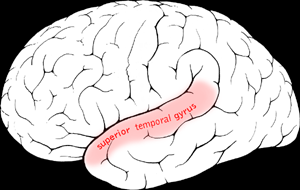
\includegraphics[width=\textwidth]{einleitung/stg.png}}
    \subcaption{Gyrus temporalis superior (STG), enthält den auditorischen Kortex. Verwendet von Auditory cortex. (18. März 2015). In Wikipedia, The Free Encyclopedia. Abgerufen 19:47, 04. August 2015, von \url{https://en.wikipedia.org/w/index.php?title=Auditory_cortex&oldid=653871107}}
    \label{img:gyrustemp}
  \end{subfigure}\hspace*{0.04\textwidth}
  %
  \begin{subfigure}[c]{0.47\textwidth}
    \fbox{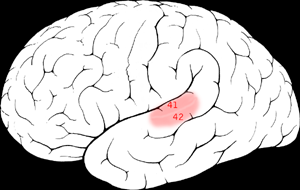
\includegraphics[width=\textwidth]{einleitung/brodmann-41-42.png}}
    \subcaption{Auditorischer Kortex in den Brodmann Arealen 41 und 42. Verwendet von Superior temporal gyrus. (20. Juli 2015). In Wikipedia, The Free Encyclopedia. Abgerufen 19:57, 04. August 2015, von \url{https://en.wikipedia.org/w/index.php?title=Superior_temporal_gyrus&oldid=672262435}}
    \label{img:audicort}
  \end{subfigure}
  %
  \vspace*{3mm}
  \caption{Gyrus temporalis superior (STG) und auditorischer Kortex}
  \label{img:audi}
\end{figure}

Der auditorische Kortex ist ein bestimmter Bereich des Gehirns. Er befindet sich an den Brodmann Arealen 41 und 42, dargestellt in Abbildung \ref{img:audicort}. Der auditorische Kortex ist Teil des Gyrus temporalis superior (STG, sieh Abbildung \ref{img:gyrustemp}), welcher bei jeglicher auditiver Stimulation aktiviert wird \parencite{binder1994functional}. Im auditorischen Kortex erfolgt dann das Bewusstwerden akustischer Signale \parencite{jaaskelainen2004human}.

In den vorliegenden Daten handelt es sich um ein auditives Experiment, weshalb die ERF (v.a. die MMN) im auditorischen Kortex erwartet werden.

% ###########################
% ##### GRUNDLAGEN MEG  #####
% ###########################

\subsection{Grundlagen der Magnetenzephalographie}

Das MEG (Magnetenzephalographie) misst die magnetischen Aktivität des Gehirns. Es ist das zweitjüngste Verfahren zur Messung der Gehirnströme. Nachdem in den 1920er Jahren das EEG durch Hans Berger entwickelt und 1929 erstmals publiziert wurde \parencite{berger1929elektrenkephalogramm}, folgte das MEG erst 1968 \parencite{cohen1968magnetoencephalography}, war damit aber noch vor anderen Verfahren zur Vermessung des Gehirns, wie dem CT (Computertomographie) oder dem MRT (Magnet-Resonanz Tomographie). Trotzdem ist das MEG auf Grund seiner hohen Empfindlichkeit, seiner damit verbundenen hohen Rauschanfälligkeit und ebenso auf Grund seines noch unausgeschöpften Lokalisations-Potentials auch heute noch ein Verfahren, welches sich in einem kontinuierlichen Optimierungsprozess befindet.

Da die Kosten eines MEG deutlich über denen eines EEG liegen, stellt sich die berechtigte Frage warum überhaupt die magnetische Komponente der Nervenzellen-Aktivität gemessen wird. Zusätzlich lassen sich mit MEG nur die tangentialen Komponenten der Aktivität messen, während EEG sowohl tangentiale, als auch radiale Aktivität erfassen kann. Die Vorteile des MEG liegen jedoch in einer geringeren Störung der magnetischen Signale durch den Schädel und die Kopfhaut, und einer damit verbundenen höheren räumliche Auflösung. Während das EEG also mehr Aktivität erfassen kann, ist das MEG präziser in der Erfassung und ermöglicht eine genauere Lokalisation. Zusätzlich ist die zeitliche Auflösung unterhalb einer Millisekunde $< 10^{-3}\,s$, die hohe Anzahl der Kanäle und die genaue Kenntnis über die Position der Kanäle (auf Grund des starren MEG-Helms) wichtige Vorteile des MEG zur Lokalisation der Quellen  \parencite{malmivuo2012comparison}.

\subsubsection{SQUIDs}
\label{sec:squids}

Technische Grundlage der Magnetenzephalographie bilden SQUIDs (Superconducting Quantum Interference Device, dt.: Supraleitende Quanteninterferenzeinheit), welche 1964 in den Ford Research Labs entwickelt wurden \parencite{jaklevic1964quantum}. Sie basieren auf dem Josephson Effekt, der bereits 1962 von Brian D. Josephson vorhergesagt wurde \parencite{josephson1962possible}. Josephson sagte voraus, dass zwei Supraleiter, welche durch eine wenige Nanometer dicke nicht-supraleitende Schicht getrennt werden (Josephson-Kontakt) und mit einem geringen elektrischen Strom durchflossen werden, von Cooper-Paaren derart durchtunnelt werden können, dass sich der Josphson-Kontakt wie ein unterbrechungsfreier Supraleiter verhält. Die Cooper-Paare tunneln in dem Fall widerstandsfrei.
Auf Grund der Cooper-Paare sind die Wellenfunktion zweier Elektronen gekoppelt (abhängig von der dicke der Schicht). Mit den Wellenfunktionen $\Psi_1$, $\Psi_2$ und den Hamilton-Operatoren $H_1$, $H_2$, sowie dem Kopplungskoeffizienten $T$ gilt:

\begin{subequations}
\label{eq:cooper}
  \begin{equation} i\hbar \frac{\partial \Psi_1}{\partial t} = H \Psi_1 + T \Psi_2 \end{equation}
   \begin{equation} i\hbar \frac{\partial \Psi_2}{\partial t} = H \Psi_2 + T \Psi_1 \end{equation}
\end{subequations}

Die erste Josphson-Gleichung beschreibt die Abhängigkeit des Stroms im Supraleiter $I_S$ vom kritischen Strom $I_0$, wobei $\Delta \phi$ die Phasendifferenz zwischen den zwei Wellengleichungen \ref{eq:cooper} bezeichnet.

\begin{equation}
\label{eq:joseph}
I_S = I_0\,\sin{\Delta \varphi}
\end{equation}

Gleichung \ref{eq:joseph} gilt jedoch nur für Prozesse ohne Magnetfeld. Sobald ein Magnetfeld anliegt, muss die Gleichung korrigiert werden. Es liegt eine Abhängigkeit des Strom im Supraleiter $I_S$ vom anliegenden Magnetfeld $\vec{B}$ bzw. vom zugehörigen magnetischen Vektorpotential $\vec{A}$ vor:

\begin{equation}
\label{eq:josephfeld}
I_S = I_0\,\sin{\left( \Delta \varphi - \frac{2\pi}{\Phi_0} \int_{S1}^{S2} \vec{A}\,d\vec{l} \right)}
\end{equation}

Der zweite Term ergänzt Gleichung \ref{eq:joseph} um ein Wegintegral vom ersten Supraleiter $S1$ über den Josephson-Kontakt zum zweiten Supraleiter $S2$. $\Phi_0$ entspricht dem Flussquant (siehe auch Gleichung \ref{eq:flussquant}).

Ein SQUID basiert auf diesem Prinzip und enthält zwei Josephson-Kontakte, in welchem ein Gleichsstrom fließt (DC SQUID) oder einen Josephson-Kontakt, in welchem ein Wechselstrom fließt (RF SQUID). Die Leiter in einem SQUID sind zu einem Ring zusammengeschlossen. Entscheidend ist, dass sich der Strom innerhalb des SQUID abhängig vom äußeren Magnetfeld verhält, wie in Gleichung \ref{eq:josephfeld} gezeigt. Das anliegende Magnetfeld kann auf einzelne Flussquanten genau angegeben werden. Ein Flussquant entspricht:

\begin{equation}
\label{eq:flussquant}
\Phi_0 = \frac{h}{2e} \approx 2,068\,Tm^2
\end{equation}

Die magnetische Flussdichte der Gehirnaktivität liegt im Bereich von wenigen $10^{-15}\,T$ und kann daher nur mit hochsensiblen Sensoren gemessen werden. Zum Einsatz kommen daher SQUIDs. Diese werden als Gradiometer oder Magnetometer eingesetzt.

\subsubsection{Gradiometer und Magnetometer}

Magnetometer besitzen nur einen SQUID-Ring und messen den absoluten Wert der magnetischen Flussdichte in radiale Richtung $B_z$ in $T$. Neben der hohen Sensitivität gegenüber nahen Quellen, wie magnetische Aktivität im Gehirn, erfassen Magnetometer auch Signale aus weiter Entfernung und damit ungewünschte Aktivität aus der Umgebung \parencite{hansen2010meg}.

Gradiometer besitzen einen zusätzlichen SQUID-Ring. Die zwei Ringe eines Gradiometers können axial oder planar angeordnet sein. Die zwei Spule messen einen räumlichen Gradienten, der Gradient der magnetische Flussdichte $G_x = dB_z/dx$ bzw. $G_y = dB_z/dy$ wird in $T/m$ angegeben. Die Annahme ist, dass weit entfernte Quellen ein relativ homogenes Feld erzeugen. Da die zwei SQUIDs des Gradiometers mit einem entgegengesetzten Strom durchflossen werden und die gemessenen magnetischen Flussdichten voneinander subtrahiert werden, verschwindet der Gradient für weit entfernte Quellen im Idealfall, so dass nur nahe Quellen erfasst werden \parencite{hansen2010meg}.

\subsection{Artefakte und Rauschen}

Wie bereits im Abschnitt \nameref{sec:squids} auf Seite \pageref{sec:squids} deutlich wurde, ist das MEG ein äußerst empfindliches Messinstrument, welche im Bereich einzelner Flussquanten $\Phi_0$ messen kann. Ziel ist es nur die Gehirnsignale zur weiteren Berechnung zu verwenden und alle anderen Störfaktoren auszuschließen. Dafür kann eine Reihe von Maßnahmen getroffen und entsprechende Software eingesetzt werden, die im Folgenden erläutert wird.

\subsubsection{Allgemeine Rauschunterdrückung}

Prinzipiell können unterschiedliche Artefakte und Rauschfaktoren ausgemacht werden. Grob können drei Bereiche klassifiziert werden: (1) Umwelt, (2) Versuchsperson und (3) Messtechnik.

Am besten zu beeinflussen ist der Faktor der Umwelt (1). Innerhalb von Städten ist beispielsweise viel bewegtes Metall (z.B. Autos, Straßenbahnen), welches zu schwachen, aber deutlich messbaren Magnetfeldern führt. Zusätzliche treten viele periodische elektrische und magnetische Felder auf (z.B. Netzkabel, Oberleitungen). All diese Faktoren können durch eine entsprechende Standortwahl deutlich verringert werden. Die verbleibenden Faktoren können durch ein stark geschirmten Messraum weiter verringert werden. Verbleibende Faktoren sind meist trotzdem deutlich in den Messungen sichtbar (z.B. Netzkabel im Gebäude).

Auch die Versuchsperson (2) hat einen großen Einfluss auf die Messung. Bewegung der Augen, Herzschläge und Kopfbewegungen, allgemein jede Kontraktion eines Muskels, führt zu deutlich messbaren mehr oder weniger periodischen Artefakten. Durch ein gutes Versuchsdesign und eine professionelle Einweisung können einige dieser Faktoren verringert werden, letztlich ist die Disziplin der Versuchsperson jedoch der entscheidende Faktor.

Letztlich hat auch die Messtechnik (3) in Form klassischen Rauschens einen entscheidenden Einfluss, maßgeblich durch Sensorrauschen.

\textcite{vigario1998independent} und \textcite{vigario2000independent} fassten mit Hilfe einer ICA (Independent Component Analysis) die wichtigsten Faktoren für Rauschen und Artefakte bei MEG-Messungen zusammen.

\subsubsection{Softwareseitige Rauschunterdrückung}
\label{sec:maxfilter}

Nachdem das Rauschen bereits während der Messung versucht wird so gut wie Möglich zu unterdrücken, kann auch auf Softwareebene nachgearbeitet werden. Eine Möglichkeit bietet die \emph{Signal-space projection} (SSP), für die eine Leerraummessung notwendig ist. Eine andere rechenintensivere Möglichkeit bietet die proprietäre Software Maxfilter von Neuromag (siehe auch Abschnitt \nameref{sec:software} auf Seite \pageref{sec:software}), die \emph{Signal-Space Separation} (SSS) zur Trennung äußerer und innerer Quellen anwendet. Mit \emph{Movement Correction} (MC) können zusätzlich die Bewegungen der Versuchsperson nachträglich korrigiert werden.

Der Signalraum (signal-space) ist ein $n$-dimensionaler Raum, wobei $n$ der Anzahl der Kanäle entspricht. Ein Vektor bzw. ein Punkt im Signalraum entspricht einem vollständigen Signal zu einem Zeitpunkt. Das räumliche Muster des Signals entspricht der Richtung des Vektors, die Intensität des Signals entspricht dem Betrag des Vektors \parencite{hansen2010meg}.

SSP wurde Ende der 90er Jahre von \textcite{uusitalo1997signal} und \textcite{parkkonen1999interference} entwickelt. Die Methode basiert auf dem Vorliegen einer Leerraummessung. In einer kurzen Messung werden die üblichen magnetischen Aktivitäten im Messraum aufgezeichnet, ohne dass eine Versuchsperson anwesend ist. Das Ergebnis entspricht den Umwelt-Artefakten, die als zeitlich konstant angesehen werden und zu jeder späteren Messung vorhanden sind. Wird eine Messung mit Versuchsperson durchgeführt, so bildet die Leerraummessung einen Unterraum des gewöhnlichen Signalraums. Durch eine orthogonale Projektion des Signalraums auf den Unterraum der Leerraumessung, ergibt sich ein weiterer Unterraum, der die Signale ohne die Umwelteinflüsse enthalten sollte. Jegliche äußeren Artefakte werden damit entfernt oder zumindest drastisch reduziert.

SSS wurde wenige Jahr später von \textcite{taulu2004suppression} und \textcite{taulu2005presentation} entwickelt. Dabei wird das gemessene Magnetfeld in einer Reihenentwicklung beschrieben. Die Entwicklung trennt sich in positive und negative Terme. Die negativen Terme ??? entsprechen im Idealfall den äußeren Signalen und können ausgelassen werden. Das Signal wird separiert in einen inneren Teil (innerhalb des MEG-Helms) und einen äußeren Teil (außerhalb des MEG-Helms). Der innere Teil wird als rauschfrei angenommen. Diese Methode ist deutlich rechenaufwändiger, führt jedoch zu deutlich rauschfreieren Ergebnissen. Zusätzlich ist keine Leerraummessung notwendig. Die Methode kann durch die angesprochene Movement Correction (MC) erweitert werden. Im normalen SSS-Verfahren wird angenommen, dass die Versuchsperson während eines Durchgangs (Block) unbewegt sitzen bleibt. Die Kopfpositionen werden nur zwischen den Blöcken auf die Position zu Beginn der Messung korrigiert. Bei der zusätzlichen MC-Berechnung wird die Kopfposition für jeden Zeitpunkt korrigiert. Zur Erfassung der Kopfposition sind Spulen am Kopf angebracht, welche zu jedem Zeitpunkt die Position der Versuchsperson erfassen. Eine zusätzliche nachträgliche Korrektur der Kopfposition ist vor allem dann sinnvoll, wenn sich die Versuchsperson sehr viel bewegt hat. Die Notwendigkeit dieses Rechenschritts kann mit Bewegungsprofilen abgeschätzt werden.

% ####################################
% ##### GRUNDLAGEN LOKALISATION  #####
% ####################################

\subsection{Grundlagen der Quelllokalisation mit MEG}

Die Messung der magnetischen Signale ausschließlich über die außerhalb des Kopfes befindlichen Sensoren. Die entscheidende Frage ist also: Wie ist es möglich anhand der magnetischen Signale außerhalb des Gehirns auf die physiologischen Quellen innerhalb des Gehirns zu schließen? Um diese Frage zu beantworten wird zunächst etwas Theorie eingeführt und anschließend die Vorwärts-Lösung, sowie verschiedene Methoden der inversen Lösung erläutert.

\subsubsection{Superposition}

Jede Quelle im Gehirn wirkt auf alle Sensoren an der Kopfoberfläche, jeder Sensor empfängt also Signale jeder einzelnen Aktivität im Gehirn. Es liegt eine Superposition der Quellaktivität vor (siehe Abbildung ???). Ähnlich einer Unterhaltung mit 10 sprechenden Personen und 5 aufnehmenden Mikrofonen. Jedes Mikrofon empfängt aus einer anderen Perspektive alle 10 Gespräche. Wünschenswert wäre es nun ein einzelnes Gespräch zu isolieren \emph{und} zu lokalisieren. Übertragen auf das Gehirn soll versucht werden die Quellen der Aktivitäten zu identifizieren und deren spezifische Aktivitäten über die Zeit zu erhalten. Die Quellen werden durch Dipole beschrieben und diskretisiert. Entsprechend soll für jeden angenommenen Dipol (an einem bestimmten Ort im Gehirn) ein Aktivitätsverlauf über die Zeit berechnet werden.

\subsubsection{Segmentierung}

Die Quellbestimmung ist nur an bestimmten Stellen innerhalb des Kopfes wirklich sinnvoll, außerhalb des Gehirns ist kein magnetischer Dipol zu erwarten. Außerdem ist es wünschenswert die Aktivität im Gehirn nicht auf eine standardisierte mathematische Form (z.B. auf eine Kugel) zu berechnen, sondern ein echtes Gehirn zu verwenden, im Idealfall das tatsächliche Gehirn der entsprechenden Versuchsperson. Dafür muss zunächst ein bildgebendes Verfahren eingesetzt werden. Überlicherweise eignet sich dafür ein MRT-Scan des Kopfes.

Das Bild des Kopfes enthält zunächst noch keine Informationen über physiologische Bestandteile. Mit dem Softwarepaket Freesurfer ??? kann das Bild des Kopfes in seine Segmente zerlegt werden. Es wird unterschieden zwischen der Kopfhaut, dem Knochen, dem Bindegewebe und dem Gehirn ???. Innerhalb des Gehirns werden Gyri und Sulki ???, sowie graue und weiße Substanz ??? getrennt.

\subsubsection{Koregistrierung}

Die Daten der Physiologie aus der MRT-Messung und die Daten der Aktivität aus der MEG-Messung werden in unterschiedlichen Räumen erhoben, da beide Verfahren mit unterschiedlichen Geräten und unterschiedlichen Standards arbeiten (auch herstellerspezifisch). Dies macht sich bei der Verarbeitung der Daten vor allem in der Wahl des Koordinatensystems bemerkbar.

Die physiologischen Daten des MRT lagen im ???-Koordinatensystem vor, während die Aktivitätsdaten des MEG im ???-Koordinatensystem vorlagen. ?? Koordinatensysteme beschreiben, evtl. auch andere ??

Bei der \emph{Koregistrierung} wird eine Koordinatentransformaition durchgeführt, so dass beide Datensätze möglichst gut zueinander passen. Die Abweichungen liegen im Bereich von ???.

\subsubsection{Volumenleiter und Quellraum}

Begrifflich wird strikt getrennt zwischen den Sensoren (sensors), welche über der Kopfoberfläche liegen und die Signale aufnehmen. Die Sensoren werden auch als Kanäle (channels) bezeichnet, vor allem dann wenn es um die mathematische Auswertung geht. Die Kopfoberfläche (headshape) bezeichnet den äußeren Rand des Kopfes. In diesem Zusammenhang wird auch der Begriff des Kopfmodells (head model) verwendet, welcher ein gesamtes Modell des Kopfrandes darstellt. Oft ist es sinnvoll auch diesen darzustellen, um z.B. die Korrektheit der Positionen von Sensoren und Kopf oder Gehirn und Kopf einschätzen zu können. Der Volumenleiter besteht ausschließlich aus dem Gehirnvolumen. Alle weiteren Teile des Kopfes wurden nach der Segmentierung verworfen. Es wird beim Volumenleiter also nur der Bereich des Kopfes betrachtet, in dem elektrische bzw. magnetische Signalquellen erwartet werden, also ein Volumen elektrisch leitenden Gewebes. Dabei wird nur beschrieben wie sich elektrische Aktivität im Gehirn verteilen kann, der Volumenleiter trifft keine Aussage über mögliche Ursprünge elektrischer Aktivität. Für jede Stelle im Gewebe wird angegeben wie hoch die Leitfähigkeit ist. Der Volumenleiter ist Resultat der Segmentierung ???.

?? Quellraum ???

?? Zusammenbringen mit nächsten Abschnitt ??

\subsubsection{Vorwärtsmodell - BEM und FEM}

Das \emph{Vorwärtsmodell} (\emph{forward solution}) berechnet aus angenommenen Quellen innerhalb des Gehirns die Auswirkung auf die Sensoren außerhalb des Gehirns. Der Rand des modellierten Gehirns wird dabei als \emph{BEM-Netz} mit Dreiecken modelliert. Die Auflösung der Modellierung sollte nicht zu gering ausfallen, da die Dipole (elementare Quellen im Gehirn) nahe der Oberfläche (bzw. nahe des BEM-Netzes) bei der numerischen Berechnung fehlerhaft berechnet werden können ?? warum ??. Eine höhere Auflösung ermöglicht eine höhere Fehlerfreiheit für Dipole nahe der Volumen-Oberfläche. In dieser Analyse wurde ein Auflösung von XXXX gewählt. ?? letzter Satz evtl. erst in Methodik ??

Innerhalb der Oberfläche befindet sich das Gehirngewebe. Die Leitfähigkeit des Gehirns wird im BEM-Modell als homogen und isotrop angenommen. Dies stellt eine Idealisierung da, im Abschnitt XX (Gehirnstruktur) wurde bereits deutlich, dass eine homogene Leitfähigkeit nicht der Realität entspricht bzw. nur für die graue Substanz gültig ist. Da die graue Substanz jedoch außen liegt und meist auch nur die Aktivitäten im Außenbereich berechnet werden, ist die Näherung meist gerechtfertigt.

Innerhalb des Volumenleiters werden Dipole modelliert (hier 10242 pro Hemisphäre ?? evtl. erst in Methodik ??). Für jeden der gesetzten Dipole wird unter Berücksichtigung der Leitfähigkeit und des Randes die Wirkung auf die Sensoren außerhalb des Gehirns bestimmt. Somit kann für viele Positionen im Gehirn die Wirkung außerhalb des Gehirns abgeschätzt werden.

Die Daten des Vorwärtsmodells werden in einer \emph{Leadfield-Matrix} gespeichert. Sie enthält die Abbildung der Dipole auf die Sensoren (numSensoren X numDipole). Durch sie wird die Berechnung des Rückwärtsmodells möglich (siehe Abschnitt ???).

\[ L = S \times D ?? \]

Im Gegensatz zum BEM-Modell wird im FEM-Modell (\emph{Finite Element Model}) angenommen, dass die Leitfähigkeit anisotrop ist. Dies entspricht mehr der Realität und lohnt sich vor allem bei einer Lokalisation, welche auch das innere des Gehirns berücksichtigt, da die weiße Substanz mit ihrer anisotropen Leitfähigkeit besser modelliert  wird.

\subsubsection{BEM-Netz und Headmodel}

?? Wo hin damit ??

Während das BEM-Netz eine glatte Oberfläche der Begrenzung des Gehirns darstellt (quasi die Kopfhaut), wird im Headmodel der Kortex mit seinen Faltungen dargestellt. Die Daten des Headmodels bilden den Sourcepace (oder Quellraum), also dasjenige Volumen, in welchem das Gewebe des Gehirns liegt und in welchem Aktivitäten dargestellt werden sollen.

\subsection{Rückwärtsmodell}

Das \emph{Rückwärtsmodell} (\emph{inverse solution}) schätzt die Aktivitätsquellen im Gehirn. Die Berechnung des Rückwärtsmodells setzt das Vorwärtsmodell voraus. Nur wenn bekannt ist wie sich bestimmte Quellen im Gehirn auf die Sensoren außerhalb des Gehirns auswirken, kann berechnet werden wie bestimmte Aktivitätsmuster an den Sensoren mit Quellen im Gehirn zusammenhängen. Für das Rückwärtsmodell können verschiedene Verfahren verwendet werden. In dieser Untersuchung werden die zwei Verfahren “Minimum Norm” und “Beamforming” verglichen.
Datenmodell
% Echte Formeln (mit Nummern) verwenden
\begin{equation}
X = h_1 s_1 + h_2 s_2 + ... + h_n s_n + R
\end{equation}

$X$ bezeichnet die Gesamtheit der Daten. Diese setzte sich zusammen aus einer linearen Summe der Quellaktivitäten si multipliziert mit den jeweils passenden Leadfield-Werten hi (siehe Abschnitt XX, Vorwärtsmodell) und dem Rest-Rauschen R.

\subsubsection{Methoden zur Bestimmung des Rückwärtsmodell}

Es gibt drei Verfahren zur Bestimmung des Rückwärtsmodells (siehe auch Abbildung XX):

\begin{itemize}
\item Einfache und multiple Dipolmodelle (single and multiple dipole models)
\item Verteilte Dipolmodelle (distributed dipole models)
\item Räumliche Filterung (spatial filtering)
\item Einfache und multiple Dipolmodelle
\end{itemize}

In den einfachen und multiplen Dipolmodellen (single and multiple dipole models) werden nur wenige Quellen angenommen, die einen großen Teil der Varianz in den Daten erklärt. Es wird zunächst ein Diopol innerhalb des Volumenleiters betrachtet und so lange variiert, bis er einen großen Teil der Varianz der Aktivität an der Kopfoberfläche bzw. an den Sensoren erklärt. Dieses Verfahren wird für einige wenige Dipole wiederholt. Je mehr Dipole verwendet werden, desto höher wird die erklärbare Varianz und desto mehr Lokalisationen können vorgenommen werden. Gleichzeitig ist die zusätzlich erklärte Varianz für jeden neuen einzelnen Dipol immer geringer, weshalb es sich nur lohnt eine überschaubare Anzahl an Dipolen zu betrachten und im Umkehrschluss nur von einer geringen Anzahl an Dipolen auszugehen.

In dieser Methode wird versucht den Fehler $R$ zwischen Daten $X$ und Modell $\sum^n_1{h_i s_i}$ so gering wie möglich zu halten. Dafür wird das Ergebnis des Modells von den Daten abgezogen, der Fehler bzw. das Rauschen bleibt übrig. Dabei wird versucht $n$ klein zu halten.

\begin{equation}
X - h_1 s_1 - h_2 s_2 - ... - h_n s_n = R
\end{equation}

\subsubsection{Verteilte Dipolmodelle}

Im verteilten Dipolmodellen (distributed dipole models) wird davon ausgegangen, dass die Aktivität überall auftritt. Es wird nach der Verteilung der Aktivität im gesamten Gehirn gesucht.

Mit der Leadfield-Matrix $H$ und den Daten ergibt sich direkt die Quellaktivitätsmatrix S:

\begin{equation}
H^{-1} ( X - R ) = S
\end{equation}

Bei den verteilten Dipolmodellen werden sehr viele Quellen betrachtet, deutlich mehr als Sensoren verfügbar sind. Damit ergeben sich unendlich viele exakte Lösungen. Um physikalisch sinnvolle Lösungen zu finden müssen Nebenbedingungen aufgestellt werden. Übliche Nebenbedingungen sind:

\begin{itemize}
\item Maximale Glättung, LORETA (maximal smoothness)
\item Minimale Energie, L2 (minimum power)
\item Minimale Amplitude, L1 (minimum amplitude)
\end{itemize}

Dabei entspricht $L2$ der $L2$- bzw. der Euklidischen-Norm. Es wird anschaulich diejenige Lösung genommen, für die die Gesamtenergie des Gehirns minimal wird.

\begin{equation}
||x||_2 = \sqrt(\sum |x_i|^2)
\end{equation}

$L1$ entspricht der $L1$- bzw. Betragssummen-Norm. Es wird anschaulich diejenige Lösung genommen, für die die Gesamtamplitude des Gehirns minimal wird.

\begin{equation}
||x||_1 = \sum |x_i|
\end{equation}

\subsubsection{Räumliche Filterung}

Bei der räumlichen Filterung (spatial filtering) werden die Zeitverläufe der Aktivitäten der einzelnen Dipole als unkorreliert betrachtet. Es wird davon ausgegangen, dass die Dipole sich nicht gegenseitig beeinflussen. Gesucht wird nach der Aktivitätswahrscheinlichkeit an jedem Punktl. Dafür wird das gesamte Gehirn mit Hilfe eines einzigen Dipols abgescannt. Unterschiedliche Verfahren stehen zur Verfügung:

\begin{itemize}
\item Beamforming, z.B. LCMV, SAM, DICS
\item Multiple Signal Classification, MUSIC
\end{itemize}

Es wird immer nur ein Ort zu einer Zeit betrachtet, die anderen Orte werden außen vor gelassen. Für den ersten Ort ergibt sich damit:

\begin{equation}
X = h_1 s_1 + N
\end{equation}

Dabei bezeichnet $N$ diejenige Aktivität, welche von allen anderen Orten außer von $s_1$ kommt.

\begin{equation}
N = h_2 s_2 + ... + h_n s_n + R
\end{equation}

Allgemein kann die Gesamtaktivität somit von jedem beliebigen Ort beschrieben werden:

\begin{equation}
X = h_i s_i + N
\end{equation}

$N$ wird also als unkorreliert mit $s_i$ betrachtet. Kommt es zu Korrelationen, so können die Quellen nicht mehr auseinandergehalten werden (van Veen, 1997).

Um jede einzelne räumliche Position betrachten bzw. berechnen zu können, wird ein räumlicher Filter benötigt. Mit diesem lässt sich die Quellaktivität mit den Daten bestimmen. Der räumliche Filter erfüllt maßgeblich zwei Funktionen:

Alle Aktivität am untersuchen Ort soll vollständig durchgelassen werden
Rauschen und andere Aktivitäten anderer Orte soll vollständig unterdrückt werden

Da der räumliche Filter nicht ideal gestaltet ist, d.h. das Signal am betrachteten Ort nicht vollständig erhalten bleibt und das Signal von allen anderen Orten inkl. Rauschen nicht vollständig unterdrückt wird, entspricht das vorhergesagte Signal nicht dem ursprünglichen Signal. Das vorgesagte Signal ist gegenüber dem ursprünglichen Signal weniger scharf.

Die Vorhersage mit Hilfe des räumlichen Filter kann und muss mathematisch beschrieben werden. Zunächst wird vom normalen Modell ausgegangen. 

\begin{equation}
X = h \cdot s \quad \text{(Daten = Leadfield-Matrix * Quellaktivität)} \; (1) \\
\end{equation}

Gleichzeitig ist das Ziel die Quellaktivität mit Hilfe des räumlichen Filters vorherzusagen:

\begin{equation}
w^T \cdot X = \hat s \quad \text{(Räumlicher Filter, transponierte Matrix * Daten = Quellaktivität)} \;(2)
\end{equation}

(1) eingesetzt in (2) ergibt:

\begin{equation}
w^T \cdot h \cdot s = \hat s \;(3)
\end{equation}

Werden die Bedingungen des räumlichen Filters als Ideal angenommen, dann entspricht die wahre Quellaktivität der vorhergesagten Quellaktivität und es gilt $s = \hat s$.
Wird Gleichung (3) durch s geteilt und obere Gleichheit angenommen, so gilt:

\begin{equation}
w^T \cdot h = 1	\;(4)
\end{equation}

Anschaulich bedeutet dies ein maximales Signal am gefilterten Ort. Für alle anderen Orte wird Gleichung (4) Null. Oder allgemein:

\begin{equation}
w^T_i \cdot h_j = \delta_{ij} \cdot 1
\end{equation}

mit i,j in n, wobei n der Anzahl der Orte entspricht.

Vorteile:

\begin{itemize}
\item Keine a priori Annahme über die Quellkonfiguration
\end{itemize}

Limitierungen (später Vergleich mit minimum norm):

\begin{itemize}
\item Korrelationen zwischen den Quellpunkten führt zu einer Verschmelzung der Quellen, die einzelnen Orte können nicht mehr getrennt werden (van Veen, 1997)
\item Bei der Durchführung von Beamforming macht es einen Unterschied, ob zuerst die Kovarianzmatrix berechnet und die Datenmittelung durchgeführt wird und anschließend die Quellrekonstruktion oder umgekehrt. Die Daten unterscheiden sich.
\end{itemize}

Gemeinsamer Filter (Common Filter)
Der Filter wird 
LCMV Beamformer
Das LCMV (Linearly Constrained Minimum Variance) Beamformer ist … Zeitdomäne (time domain)
Bei der LCMV Methode (van Veen et al., 1997) wird der gesamte Zeitbereich (time domain) erfasst. Ähnlich wie bei der Minimum Norm Lösung wird für jeden Zeitpunkt eine Lokalisierung über das gesamte Frequenzspektrum durchgeführt.

SAM ...

Bei der DICS Methode wird nur eine einzige Quelllösung berechnet. Es wird ein bestimmtes Zeit/Frequenz-Intervall (siehe Zeit-Frequenz-Analyse) ausgewählt. Für diesen Bereich lässt sich eine Lokalisierung bestimmen. Der Vorteil dieses Verfahrens liegt darin, dass bestimmte Bänder (z.B. Alpha-Band) genau betrachtet werden können bzgl. Lokalisierung und Aktivität.

\subsection{Leadfieldmatrix bei Beamformer und Minimum Norm}

Die Liedfield-Matrix wird für eine bestimmte Kopfposition bestimmt. Da Probanden ihren Kopf nie exakt an einem Ort halten, muss genau genommen für jede vorkommende Kopfposition bestimmt werden, wie sich in diesem Fall die Quellen auf die Sensoren auswirken (Vorwärtsmodell). Während bei den SSS- und den MC- Daten kein Problem auftritt, da hier die Kopfposition korrigiert wird, ist dies bei den Rohdaten problematischer. Bei Verwendung der Rohdaten muss also berücksichtigt werden, dass die Leadfield-Matrix nur für die initiale Kopfposition korrekt ist, alle anderen Kopfpositionen enthalten im Rückwärtsmodell entsprechende Fehler.

Vor allem bei der Bewertung des Beamformer-Verfahrens muss dieser Aspekt zwingend beachtet werden, da hier mit den Rohdaten gerechnet wird. Um einen aussagekräftigeren Vergleich zu erhalten, wäre hier eine Bewegungskorrektur nötig, die explizit keine Rauschunterdrückung durchführt. Maxfilter kann in diesem Fall also nicht verwendet werden, da die Bewegungskorrektur mit Rauschunterdrückung einher geht. Eine Implementierung eines solchen Bewegungs-Korrektur-Verfahrens könnte die Beamformer-Lösung verbessern, vor allem bei solchen Probanden, die sich viel bewegen.
Kopfkorrektur bei Rohdaten und rauschunterdrückten Daten

Das SSS-Verfahren(Signal-Space Separation) von Maxfilter beinhaltet neben der Trennung der Signale in einen inneren und einen äußeren Bereich auch eine Kopfkorrektur, da ein absolutes Stillhalten der Versuchspersonen keinen realen Versuchsbedingungen entspricht. Dabei wird die Position des Kopfes bezüglich den Sensoren standardisiert, die Kopfposition zu Beginn des ersten Blocks wird als Standard definiert. Die Signale die aus dem Gehirn kommen müssen von der gleichen Quelle aus immer auch die gleichen Sensoren ansprechen, andernfalls kommt es in der späteren Berechnung zu Fehlern. Wird eine falsche Kopfposition angenommen, werden gemessene Signale an den Sensoren später einer falschen bzw. verschobenen Quelle zugeordnet.

Während bei MC (movement correction) angenommen wird, dass der Kopf sich innerhalb eines Blocks bewegt, wird bei SSS angenommen, dass der Kopf innerhalb eines Blockes an der gleichen Position bleibt. Zwischen den Blöcken wird jedoch auch bei SSS korrigiert. Alle späteren Blöcke werden am Startpunkt auf die Position des ersten Blocks gesetzt, die Positionen der Sensoren (??) werden entsprechend umgerechnet.

Werden die SSS oder MC-Daten verwendet können im Preprocessing alle Daten, d.h. über alle Trials in allen Blöcken gemittelt werden, da die Kopfposition bereits korrigiert ist und jeder Sensor konstant die Daten desselben Ortes erfasst. Werden jedoch Rohdaten verwendet, dann ist nicht mehr sichergestellt, dass jeder Sensor die Daten des gleichen Ortes erfasst. Eine Mittelung über Rohdaten hätte zur Folge, dass eigentlich vorhandene Aktivitäten verschwinden können oder nicht vorhandene Aktivitäten auftauchen. Eine Mittelung der Trials zwischen den Blöcken kommt also zunächst nicht in Frage.

Theoretisch gibt es zwei Möglichkeiten mit Rohdaten umzugehen:

Eine Möglichkeit ist die Korrektur der Kopfpositionen, ohne jedoch eine Rauschunterdrückung vorzunehmen. So bietet FieldTrip z.B. die Funktion \texttt{ft\_megrealign}. Die Korrektur der Kopfposition erfolgt durch eine Projektion. Es wird zunächst eine grobe Quellrekonstruktion durchgeführt und es werden Standard-Positionen der Sensoren festgelegt, zum Beispiel vom Beginn des ersten Blocks. Die zeit-gemittelten Daten werden dann mit Hilfe der rekonstruierten Quelle projiziert (???). Die dabei entstehenden Signale für die standardisierte Position werden anschließend neu berechnet. Bei diesem Verfahren kommt es wegen der enthaltenen Quellrekonstruktion zu Fehlern in den Daten, die Daten sind lediglich interpoliert und enthalten nach der Korrektur nicht mehr die vollständigen Informationen. Es handelt sich nicht mehr um reine Rohdaten, weshalb dieses Verfahren nur einen Kompromiss darstellen würde.

Eine zweite Möglichkeit ist das Mitteln der Quellaktivität. Für jeden Block kann eine eigene Leadfield-Matrix für das Vorwärtsmodell bestimmt werden. Nach anschließender Quelllokalisation können die Aktivitäten an den Quellen gemittelt werden. Der Rechenaufwand ist zwar etwas erhöht, da für jeden Block die Leadfield-Matrix bestimmt werden muss, gleichzeitig bietet dieses Verfahren jedoch den Vorteil, dass es auch auf die rauschunterdrückten Daten von Maxfilter (SSS, MC) angewendet werden kann. Auch hier kann im Preprocessing absichtlich auf eine Mittelung zwischen den Blöcken verzichtet werden. Die Leadfield-Matrizen können dann auch hier blockweise bestimmt und die Quellaktivitäten am Ende gemittelt werden. Diese Möglichkeit bietet damit eine optimale Vergleichbarkeit zwischen der Verwendung von Rodaten und rauschunterdrückten Daten, unabhängig vom verwendeten Lokalisatiobsverfahren.

\newpage

\section{Methodik}

\subsection{Verwendete Daten}

Die verwendeten Daten wurden aus einem Experiment von \textcite{herrmann2011syntactic} übernommen. Dabei sollten die neuronalen Prozesse bei der Satzverarbeitung des menschlichen Gehirns untersucht werden. Die Sätze wurden dabei vorgelesen und per Kopfhörer von den Pobanden angehört. Zum einen wurden die Effekte einer syntaktischen Verarbeitung betrachtet. Sätze wurden in einer korrekten grammatikalischen Reihenfolge (Standard) oder einer falschen Reihenfolge (Deviant) präsentiert. Dabei wurde in früheren Experimenten ein ELAN (Early Left Anterior Negativity) Potential beobachtet, sofern die grammatikalische Wortfolge falsch war. Zum anderen wurden die Effekte einer räumlichen Abweichung gesprochener Sätze betrachtet. Die interaurale Laufzeit (Interaureal Time, ITD) wurde entsprechend variiert, so dass der Lautsprecher an einem Ohr relativ zum Lautsprecher am anderen Ohr die Sätze verzögert ausgab. In früheren Experimenten wurde hier eine MMN (Mismatch Negativity) beobachtet (siehe auch Abschnitt \nameref{sec:erf} auf Seite \pageref{sec:erf}).

Die beiden Effekte, die zu ELAN und MMN führen treten in Interaktion, wie \textcite{hahne2002differential} erstmals feststellten. Die Hypothese der Studie von \textcite{herrmann2011syntactic} lautete, dass die Verarbeitung dieser beiden Effekte, sofern sie gleichzeitig auftreten, im Gehirn zwar in unterschiedlichen Regionen, aber parallel verarbeitet werden.

Wie genau sieht eine Abweichung aus? Was sind Deviants???

Welche Blöcke wurden verwendet??? 1,3,4,6: Warum???

Aus den Daten waren für den Fall der vorliegenden methodischen Untersuchung vor allem die MMN von Interesse. Das Potential ist im Zeitverlauf recht deutlich zu erkennen und kann für eine Lokalisation gut verwendet werden. Zwar wird ein schlechteres Signal-Rausch-Verhältnis erwartete (siehe Abschnitt \nameref{sec:snr} auf Seite \pageref{sec:snr}), als es z.B. im Oddball Paradigma \parencite{naatanen2004mismatch} vorkommt, die verwendeten Daten basieren jedoch auf einem Experiment, welches einer realistischen bzw. alltäglichen Verarbeitung im Gehirn entspricht (Verarbeitung von gehörten Sätzen). Da es sich in dem Experiment, auf dem die verwendeten Daten basieren, um ein Experiment zur Sprachverarbeitung handelt, ist ein MMN-Potential im auditorischen Kortex zu erwarten (siehe auch Abschnitt \nameref{sec:audicort} auf Seite \pageref{sec:audicort}).

\subsection{MEG-Gerät}

Im verwendeten MEG, dem \emph{Vectorview by Elekta-Neuromag Oy, Helsinki} werden insgesamt 306 Sensoren für die Messung der Gehirnsignale verwendet. Davon sind 204 Gradiometer und 102 Magnetometer. Die Sensoren bestehen aus DC SQUIDs ... Helium ...

Neben den Sensoren zur Messung der Gehirnsignale werden weitere Sensoren zu Messung der Augenbewegung (EOG ???) und ??? verwendet.

\subsection{MRT-Gerät}



\subsection{Software zur Analyse}
\label{sec:software}

Zur Verarbeitung der vorliegenden Daten wurde verschiedene Software verwendet. Gearbeitet wurde auf einem \emph{GNU/Linux}-System mit \emph{Kubuntu} in Version ???. Die Auswertung der bildgebenden Daten des MRT erfolgte mit \emph{Freesurfer} in Version ???. Die Signal Space Separation (SSS) und Movement Correction (MC) wurde mit \emph{Maxfilter} in Version ??? durchgeführt (siehe auch Abschnitt \nameref{sec:maxfilter} auf Seite \pageref{sec:maxfilter}). Alle weiteren Analysen erfolgten mit der Open Source Paket \emph{FieldTrip} in Version ???, welches in Matlab (Version ???) verwendet wurde.

\emph{MNE} in Version ??? und \emph{Neuromag} in Version ??? 

\subsection{Verfahren}

MRT Separation, Koregistrierung, Roh/SSS/MC, MNE/LCMV + Grafik

\section{Ergebnisse}

\subsection{Signal-Rausch-Verhältnis}
\label{sec:snr}

Das Signal-Rausch-Verhältnis (signal-noise-ration, SNR) gibt das Amplitudenverhältnis der Daten an. Die Daten werden dabei in einen Rausch-Anteil $P_R$ und einen Signal-Anteil $P_S$ zerlegt. Allgemein gilt:

\begin{equation}
SNR = \frac{P_S}{P_R}
\end{equation}

Als Rausch-Anteil wurden die ersten 100 ms gewählt. Dies entspricht der Baseline. Als Signal-Anteil wurde die MMN verwendet, welche im Bereich 150 ms bis 250 ms liegt. Damit ergeben sich zwei Zeitbereiche von je 100 ms, die in den Butterfly-Diagrammen der Rohdaten (siehe Abbildungen ???) dargestellt sind. Verwendet wurden 225 der 13?? Trials pro Block, diese entsprechen der Deviant-Bedingungen, da nur hier ein Signal für die MMN erwartet wird.

Es wurden nur jene Kanäle für die Berechnung verwendet, welche am Ort der Entstehung der MMN entsprechende Signale messen. Dafür wurde zunächst das Amplitudenmaximum aus allen Trials und Zeitpunkten bestimmt. Für die zwei berechneten Versuchspersonen ergaben sich das Maximum an Kanal \texttt{MEG014} für \texttt{pa10} und Kanal \texttt{MEG151} für \texttt{pa07}. Das leicht verschobene Maximum ist auf eine unterschiedliche Position des Kopfes der Versuchsperson im MEG-Helm während des Versuchs zurück zu führen. Nachdem die Maxima bestimmt wurden, wurden die umliegenden Kanäle in die Berechnung des Signals integriert. Die verwendeten Kanäle sind:

\texttt{MEG013}, \texttt{MEG014}, \texttt{MEG021}, \texttt{MEG024}, \texttt{MEG151}, \texttt{MEG154}, \texttt{MEG152}, \texttt{MEG161}

In der Karte (Abbildung ???) wird deutlich, dass die Kanäle wie zu erwarten für die MMN im linken temporalen Bereich liegen (Stimulation erfolgte linksseitig). Von den Kanälen wurden sowohl die Magnetometer, als auch die beiden Gradiometer berücksichtigt.

Zur Berechnung des SNR wurden die Rohdaten verwendet, was eine erneute Vorverarbeitung nötig macht. Dabei wurde der gesamte Datensatz nach obigen Kriterien in die Trials zerteilt. Jeder Trail wurde anschließend in einen Rausch- und einen Signal-Anteil getrennt. Von der Baseline (Rausch-Anteil) wurde der Mittelwert gebildet.

\begin{equation}
\bar{b}_{ik} = \frac{1}{n_b} \sum_{j=1}^{n_b} b_{ijk}
\end{equation}

Dabei ist $i$ der Index der Kanäle, $j$ der Index der Zeitpunkte und $k$ der Index der Trials. $n_b$ entspricht der Anzahl der Zeitpunkt, die innerhalb der Baseline berücksichtigt werden mit $n_b = 100$. $b_{ijk}$ entspricht einer dreidimensionalen Matrix, welche die Amplituden für alle Trials, Zeitpunkt und Kanäle enthält. Gemittelt über die Zeitpunkt ergibt sich eine zweidimensionale Matrix $b_{ik}$, welche eine mittlere Amplitude für jeden Trial und jeden Kanal enthält.

Dieser Mittelwert wird für jeden einzelnen Zeitpunkt innerhalb der gesamten Aktivität (sowohl für den Rausch-Anteil, als auch für den Signal-Anteil) subtrahiert, um das mittlere Rauschen aus der Aktivität heraus zu rechnen.

\begin{equation}
\hat{b}_{im} = b_{im} - \bar{b}_{ik}
\hat{s}_{im} = s_{im} - \bar{b}_{ik}
\end{equation}

Dabei wurden die Zeitpunkt $j$ und die Trials $k$ zusammengefasst im Index $m$, eine Trennung dieser beiden Indizes ist an der Stelle nicht mehr notwendig, es handelt sich nur noch um eine Anzahl von Trials $m$. $\hat{b}_{im}$ entspricht dem korrigierten Rausch-Anteil und $\hat{s}_{im}$ dem korrigierte Signal-Anteil.

Die neuen Matrizen werden anschließend durch die Anzahl der Zeitpunkt geteilt. Dieser formale Schritt ist nötig für den Fall, dass sich die Zeitbereiche der beiden Anteile unterscheiden. In diesem Fall liegen beide bei $n_b = n_s = 100$ Zeitpunkten, so dass dieser Schritt auch ausgelassen werden könnte. Der Vollständigkeit halber:

\begin{equation}
\tilde{b}_{im} = \frac{\hat{b}_{im}}{n_b} \quad \text{und} \quad \tilde{s}_{im} = \frac{\hat{s}_{im}}{n_s}
\end{equation}

Im folgenden Schritt werden die Kovarianzenfür die beiden Anteile bestimmt.

\begin{equation}
b_{ij} = \tilde{b}_{im} \cdot \tilde{b}_{mj} \quad \text{und} \quad s_{ij} = \tilde{s}_{im} \cdot \tilde{s}_{mj}
\end{equation}

$b_{mj}$ bzw. $s_{mj}$ entspricht dabei der transponierten Matrix von $b_{im}$ bzw. $s_{im}$, wobei $i$ und $j$ jeweils den Index des Kanals bezeichnet. Die Varianzmatrizen $b_{ij}$ und $s_{ij}$ ist quadratisch und enthält die Varianzen der Amplituden zwischen allen Kanälen. Die Diagonalelemente der Matrizen entsprechen dann den Kovarianzen der Kanäle. Die Kovarianzen werden komponentenweise dividiert und anschließend gemittelt:

\begin{equation}
SNR = \sum_i \delta_{ij} \frac{s_{ij}}{b_{ij}}
\end{equation}

Für die verwendeten Daten eines auditorischen Experiments, welches auf einer komplexen Satzverarbeitung basiert ist kein sehr hohes SNR zu erwarten, es sollte jedoch oberhalb von $3$ liegen. Dieser Wert wird von der Software \emph{MNE} als Grenzwert vorgeschlagen ???.

\begin{table}[t]
\caption{}
\label{tab:snr}
\vspace*{3mm}
\begin{tabularx}{\textwidth}{cll}
Block & pa07 & pa10 \\
\hline
1 & $3.123$ & $3.915$\\
3 & $2.942$ & $3.144$\\
4 & $2.589$ & $3.875$\\
6 & $2.715$ & $3.348$\\
\hline
\end{tabularx}
\vspace*{3mm}
\caption*{Signal-Rausch-Verhältnis für zwei Versuchspersonen in jeweils 4 Blöcken. Das Verhältnis sollte im Idealfall einen Wert von $3$ überschreiten.}
\end{table}

Die Ergebnisse sind in Tabelle \ref{tab:snr} dargestellt. Deutlich wird, dass das Signal-Rausch-Verhältnis um den Wert von $3$ liegt. Während \texttt{pa07} eher leicht unterhalb von $3$ liegt, sind die Werte von \texttt{pa10} gut oberhalb von $3$. Das Signal-Rausch-Verhältnis spricht dafür, dass die Daten zur Lokalisation geeignet sein sollten, die Ergebnisse jedoch etwas verrauscht werden könnten.

\newpage
\section{Literaturverzeichnis}

\printbibliography[heading=none]

%\includepdf[pages=-]{appendix/anhang-trennblatt-versuchsaufbau.pdf}

\end{document}